
% This LaTeX was auto-generated from an M-file by MATLAB.
% To make changes, update the M-file and republish this document.

\documentclass{article}
\usepackage{graphicx}
\usepackage{color}
\usepackage{listings}
\usepackage[framed]{mcode}
\usepackage{fullpage}
\usepackage{hyperref}
\usepackage{amsmath}

\definecolor{lightgray}{gray}{0.5}
\setlength{\parindent}{0pt}

\begin{document}

    
    
\begin{par}

\title{BE 521 - Homework 1\\{\normalsize Spring 2015}}
\author{Mike Lautman}
\date{\today}
\maketitle

\end{par}
\begin{par}

\section*{1. Seizure Activity}

\end{par}
\begin{par}

\subsection*{1.1 Sampling Rate and Nyquist Freq}

\end{par}
\begin{lstlisting}
clear; clc; clf; close all;
dataset = 'I521_A0001_D002';
me = 'mlautman';
pass_file = 'mla_ieeglogin.bin';
[T,session] = evalc('IEEGSession(dataset, me, pass_file)');
data=session.data;
sample_rate = data.sampleRate % 200 Hz
nyquist_freq = sample_rate / 2 % 100 Hz
\end{lstlisting}

\color{lightgray} \begin{lstlisting}
sample_rate =

   200


nyquist_freq =

   100

\end{lstlisting} \color{black}
\begin{par}

\subsection*{1.2 Scale}

\end{par}
\begin{lstlisting}
recording_length= data.channels(1).getNrSamples;
recording_length_s = recording_length/sample_rate
vals_all = data.getvalues(1:recording_length,1);
max_value = max(vals_all)


%    In I521_A0001_D001, the sample rate was 32051 Hz, the nyquist freq was 16kHz, the
% recording lenght was 10 seconds, the voltage scale was 0.001 V, and
% the maximum value was 136.57 mv
%    In I521_A0001_D002, the sample rate was 200 Hz, the nyquist freq was 100Hz, the
% recording lenght was 645 seconds, the voltage scale was 1 V, and
% the maximum value was 2221 V.
\end{lstlisting}

\color{lightgray} \begin{lstlisting}
recording_length_s =

  644.9950


max_value =

        2221

\end{lstlisting} \color{black}
\begin{par}

\subsection*{1.3 IEEG plot}
\centering
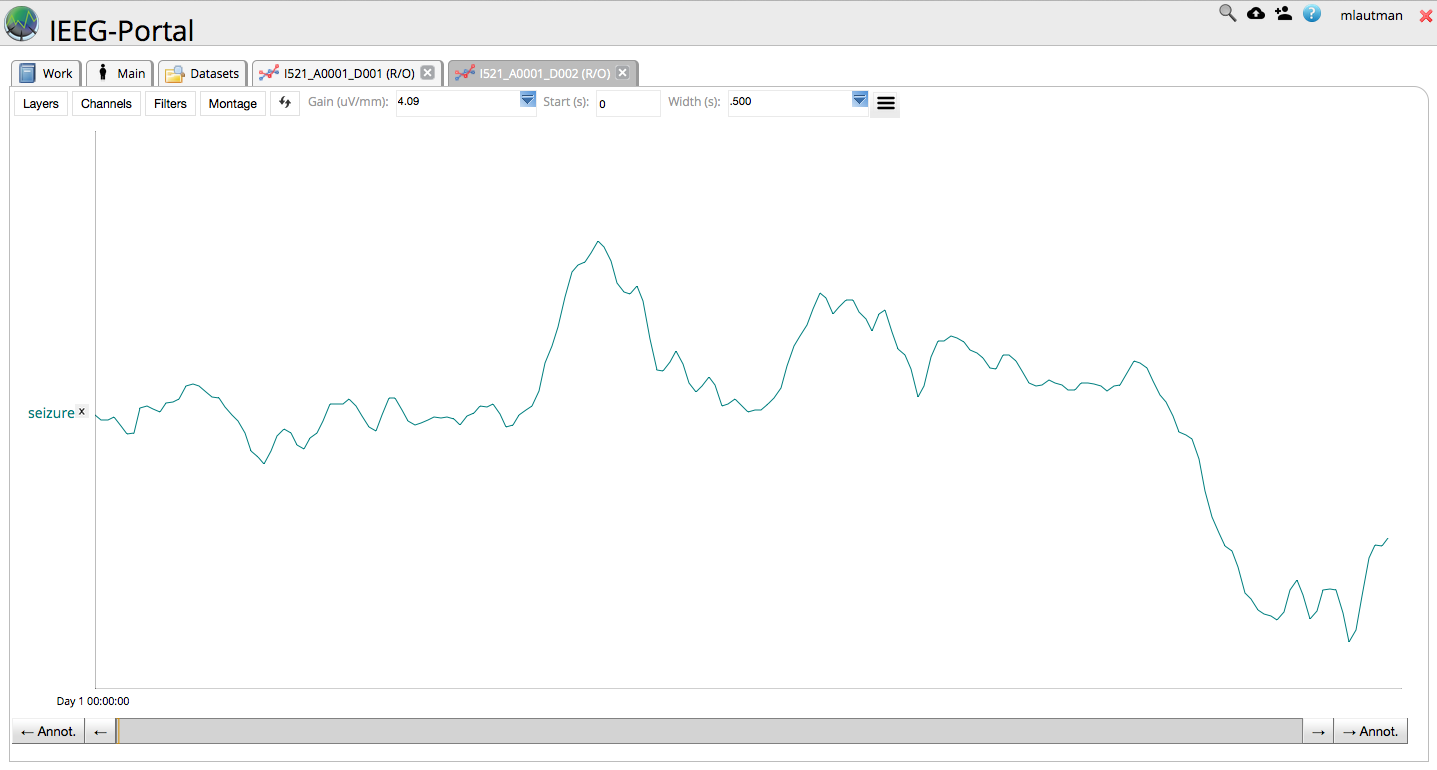
\includegraphics[width=4in]{IEEG_plot.png}
\\Figure 1. IEEG portal screenshot
\raggedright
<latex>
\subsection*{1.4 Comparing data}
The data from I521\_A0001\_D002 has much higher amplitude and more low
frequency elements. We also see there is less high frequency noise.
\subsection*{1.5 }
The bandpass filter used for I521\_A0001\_D001 would account for the
higher amplitude signal in I521\_A0001\_D002 since the low frequency
elements have the highest intensity. If we were to apply the same
bandpass to I521\_A0001\_D002, we wouldn't see so much low frequency
noise. Since the power of a frequency band scales aproxmiately with 1/f
these low frequency elements dominate much of the total signal power.
\section*{2. Evoked Potentials}
\subsection*{2.1 Using all or some of the data}
  We should crop off the first 8 pulses or 8 seconds as the stim
  amplitude durring this interval is significantly different than
  the stim amplitude durring the rest of the signal. This
  difference might affect any analysis we do on the EP signal response
  to the stimulation.
\subsection*{2.2 Bringing the EP and stim data into matlab}

\end{par}
\begin{lstlisting}
clf; clear all;

dataset2 = 'I521_A0001_D003';
me = 'mlautman';
pass_file = 'mla_ieeglogin.bin';
[T,session2] = evalc('IEEGSession(dataset2, me, pass_file)');
sample_rate2 = session2.data.sampleRate;
\end{lstlisting}



\includegraphics [width=4in]{BE521HW1_mlautman_01.png}
\begin{par}

\subsection*{2.2 Scale}

\end{par}
\begin{lstlisting}
data2 = session2.data;
recording_length2= data2.channels(1).getNrSamples;
recording_length_s2 = recording_length2/sample_rate2;
s_s = 8; % seconds
s = max(round(s_s*sample_rate2), 1);
EP = data2.getvalues(s:recording_length2,1);
stim = data2.getvalues(s:recording_length2,2);
EP_length_s = length(1:sample_rate2:length(EP)-sample_rate2);

sum_delta = 0;
% plot((s:recording_length2)./sample_rate2, EP, 'color', 'b');
% plot((s:recording_length2)./sample_rate2, stim - 5e+4, 'color', 'g');
for i=1:sample_rate2:length(EP)-sample_rate2
    interval = EP(i:i+sample_rate2);
    [m, index] = max(interval);
    sum_delta = sum_delta + index / sample_rate2;
%     plot(s_s+(i+index)/sample_rate2,m, '*', 'color', 'r');
end
ave_delta = sum_delta/EP_length_s;
ave_delta_ms = ave_delta * 1000 % 169.2 ms
\end{lstlisting}

\color{lightgray} \begin{lstlisting}
ave_delta_ms =

  169.2125

\end{lstlisting} \color{black}
\begin{par}

\subsection*{2.3 Average signal}

\end{par}
\begin{lstlisting}
EP_time_indexed = zeros(EP_length_s, sample_rate2);
cnt = 0;
for i=1:sample_rate2:length(EP)-sample_rate2
    cnt = cnt + 1;
    interval = EP(i:i+sample_rate2-1);
    EP_time_indexed(cnt, 1:sample_rate2) = interval - mean(interval);
end

EP_ave = mean(EP_time_indexed,1);
EP_std = std(EP_time_indexed,1);
T = (1:sample_rate2)./sample_rate2;
figure(1)
hold on
errorbar(T, EP_ave, EP_std, 'color', [0.7 0.7 0.7])
plot(T, EP_ave, 'color', 'r')
xlim([0,1])
ylabel('Voltage (V)', 'FontSize',10,'FontWeight','bold');
xlabel('Time (S)', 'FontSize',10,'FontWeight','bold');
title('Average EP from IEEG dataset I521\_A0001\_D003', 'FontSize',12,'FontWeight','bold');
legend('Standard Deviation from Average EP', 'Average EP');
\end{lstlisting}

\centering
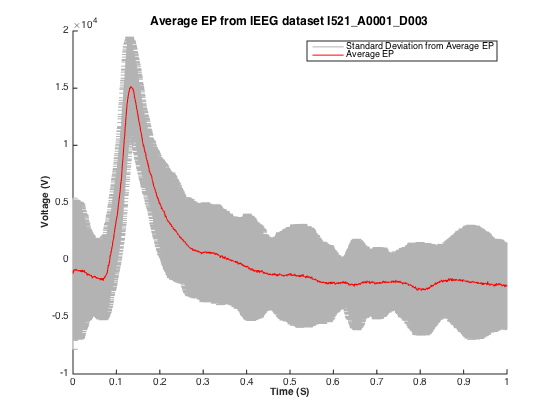
\includegraphics [width=6in]{BE521HW1_mlautman_02.png}
\\Figure 2. Average EP signal with standard deviations
\raggedright
\begin{par}

\subsection*{1.4.a characterizing signal noise}
  We know that this type of signal is composed of frequencies within a
  certain range. Frequencies above and below that range can be filtered
  to produce a 'true' signal. We can then characterize the noise as the
  magnitude of the difference between this 'true' signal and the observed
  signal.
\subsection*{2.4.b Implementing noise filter}

\end{par}
\begin{lstlisting}
figure(2)
beta = .15;
num_signals = 5;
for i=1:num_signals
    signal = EP_time_indexed(i,:);
    len = length(signal);
    signal_lpf = lpf(signal, beta);

    subplot(num_signals,3, (i-1) * 3 + 1)
    plot(1:len, signal)
    xlim([1,len])
    ylim([1.1*min(signal), 1.1*max(signal)])
    ylabel('Voltage (V)', 'FontSize',10,'FontWeight','bold');
    xlabel('Time (S)', 'FontSize',10,'FontWeight','bold');
    title('Signal', 'FontSize',12,'FontWeight','bold');

    subplot(num_signals,3, (i-1) * 3 + 2)
    plot(1:len, signal_lpf)
    xlim([1,len])
    ylim([1.1*min(signal), 1.1*max(signal)])
    ylabel('Voltage (V)', 'FontSize',10,'FontWeight','bold');
    xlabel('Time (S)', 'FontSize',10,'FontWeight','bold');
    title('LPF signal', 'FontSize',12,'FontWeight','bold');

    subplot(num_signals,3, (i-1) * 3 + 3)
    plot(1:len, (signal - signal_lpf))
    xlim([1,len])
    ylim([-5e+3, 5e+3])
    ylabel('Voltage (V)', 'FontSize',10,'FontWeight','bold');
    xlabel('Time (S)', 'FontSize',10,'FontWeight','bold');
    title('Error', 'FontSize',12,'FontWeight','bold');
end
\end{lstlisting}

\centering
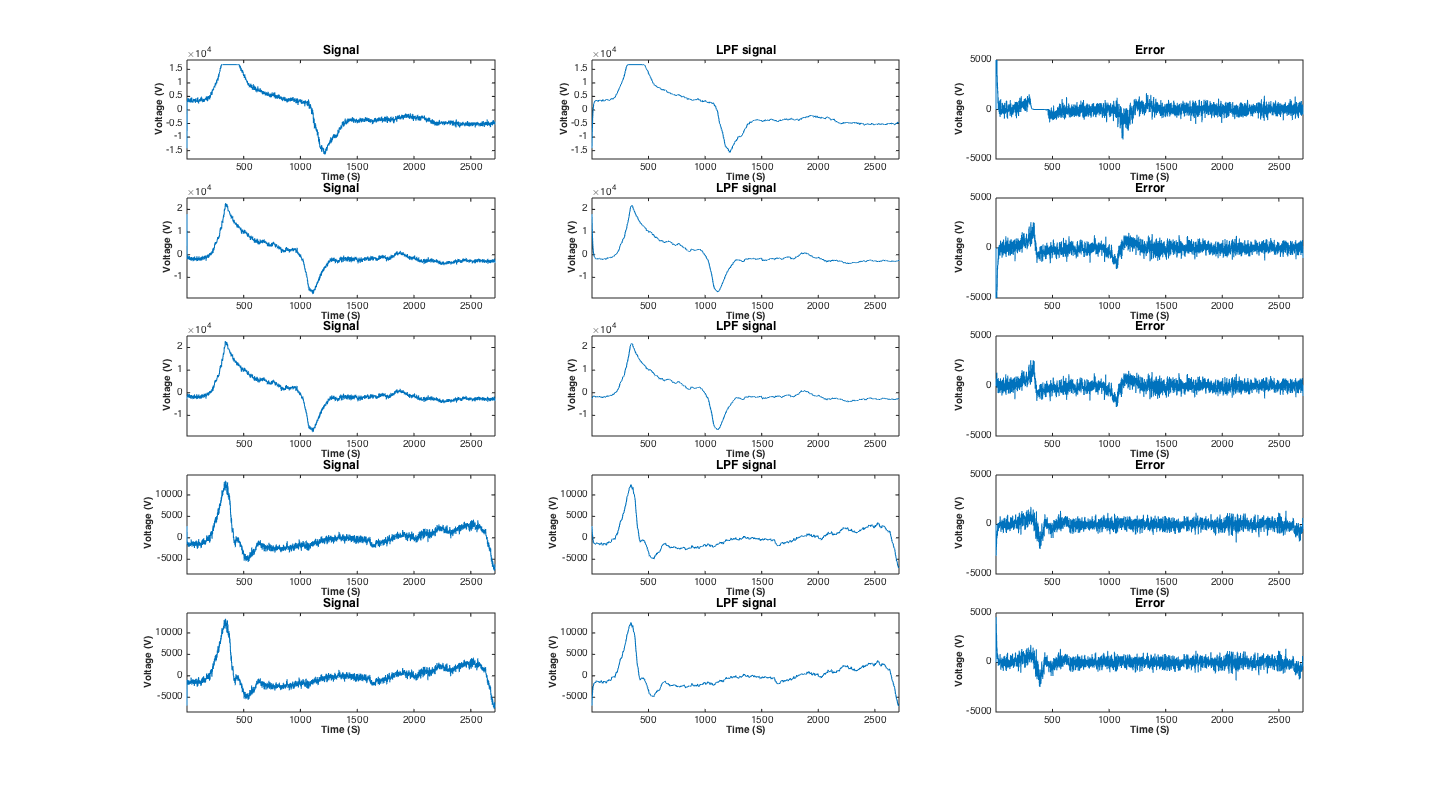
\includegraphics [width=6in]{noise.png}
\\Figure 3. Characterizing Noise using a low pass filter. 
\raggedright

\begin{par}

\subsection*{2.4.c.i Average noise}

\end{par}
\begin{lstlisting}
[signals, sig_len] = size(EP_time_indexed);
total_noise = 0 ;
for i=1:signals
    signal = EP_time_indexed(i,:);
    signal_lpf = lpf(signal, beta);

    total_noise = total_noise + norm(signal - signal_lpf);
end
average_noise = total_noise / signals
\end{lstlisting}

\color{lightgray} \begin{lstlisting}
average_noise =

   2.6497e+04

\end{lstlisting} \color{black}
\begin{par}

\subsection*{2.4.c.ii Average noise for average EP}

\end{par}
\begin{lstlisting}
EP_ave_lpf = lpf(EP_ave, beta);
EP_ave_noise = norm(EP_ave - EP_ave_lpf)
\end{lstlisting}

\color{lightgray} \begin{lstlisting}
EP_ave_noise =

   9.7826e+03

\end{lstlisting} \color{black}
\begin{par}

\subsection*{2.4.c.iii Sanity check}
These values do make sense since the averaged EP should have less noise
than the average noise of the individual EP signals.

\end{par}



\end{document}
    
